\documentclass{article}
\usepackage[hidelinks]{hyperref}
\usepackage{csquotes}
\usepackage[vmargin=25mm, hmargin=20mm]{geometry}
\usepackage{longtable}
\usepackage{array}
\usepackage[
    backend=biber,
    sorting=none,
    style=ieee,
    urldate=long,
    maxcitenames=2,
    mincitenames=1
]{biblatex}
\addbibresource{sources.bib}
\usepackage{multicol}
\usepackage{float}
\usepackage{graphicx}

\title{Looking at Challenges and Mitigation in Symbolic Execution Based Fuzzing Through the Lens of Survey Papers}

\begin{document}
% ----------
% FORMATTING 
% ----------

% Bullet list vertical spacing
\let\savedItemize=\itemize
\let\savedEndItemize=\enditemize
\renewenvironment{itemize}{\savedItemize\setlength\itemsep{0px}}{\savedEndItemize}

% Make Tables less crowded
\AtBeginEnvironment{longtable}{\renewcommand\arraystretch{1.6}}
\newcolumntype{P}[1]{>{\raggedright\arraybackslash}p{#1}}

% Column separation
\setlength{\columnsep}{13mm}

% Font size for bibliography
\renewcommand*{\bibfont}{\footnotesize}

% introduce non-breaking space before citations and references
\let\savedCite=\cite
\renewcommand{\cite}{\unskip~\savedCite}
\let\savedRef=\ref
\renewcommand{\ref}{\unskip~\savedRef}

% --------
% WARNINGS
% --------

% Disable minimally overfull hbox warnings
\hfuzz=50px

% Disable minimally underfull hbox warnings
\hbadness=1000

% ---------------
% CUSTOM COMMANDS
% ---------------

\newcommand{\tableh}[1]{\multicolumn{1}{|c|}{\textbf{#1}}} % table header
\newcommand{\code}{\texttt}
\newcommand{\papertitle}[1]{\citetitle{#1} (\citedate{#1})\cite{#1}}

\maketitle
\begin{multicols}{2}
    \begin{abstract}
        Testing is a critical and substantial part of software development. While manual testing is not scalable, automated testing in the form of fuzzing has its limitations. To enhance fuzzing's effectiveness, one approach is to combine it with program analysis techniques such as symbolic execution. However, this also presents its own set of challenges. This work utilizes survey papers on fuzzing to explore this in both academia and industry extensively studied field. %
        %
        After summarizing the focus of each paper and reviewing their discussion of symbolic execution, this work filters, collects, aggregates, and extends their analysis of the inherent challenges that symbolic execution based fuzzing faces, along with the mitigation attempts introduced by a diverse range of systems. The challenges are then categorized, and primary works and their innovations are associated with the appropriate challenge, forming an extensive list of approaches and examples. A total of 78 fuzzing systems employing symbolic execution were identified from 17 survey papers. %
        %
        This paper concludes by discussing the limitations of using survey papers to digest vast research fields and suggesting potential further analyses based on the surveyed material.
    \end{abstract}

    \section{Introduction}
    In 2022, the cost of poor software quality was estimated to be more than \$2.4 trillion in the US alone.\cite{CostPoorSoftware} Individual cyber attacks have had an estimated financial impact of up to \$8 billion worldwide.\cite{Demystifying} Software testing often accounts for more than 50\% of development costs\cite{Orchestrated}, but it is typically a mostly manual process\cite{PreliminaryAssessment}. Because manual testing requires many developer hours with in-depth knowledge of the system being tested, it does not scale well. Automated testing promises to be more cost effective in finding software defects and has therefore become the most popular vulnerability discovery solution, especially in the industry.\cite{FuzzingASurvey}

    One such automated vulnerability and bug testing technique is fuzzing.\cite{VulnerabilityDiscoveryTechniques} In the seminal work by \citeauthor{UNIX} in \citeyear{UNIX}, the term \textquote{fuzz} is defined as a program that \textquote{generates a stream of random characters to be consumed by a target program}\cite{UNIX}. Since then, a rich ecosystem of fuzzing systems has emerged in both industry and academia, taking design inspiration from a variety of software engineering concepts. These are combined into programs that generate various concrete inputs, which are then repeatedly fed into a particular program under test (PUT), and check the program for illegal states or crashes.\cite{EvaluatingFuzzTesting}

    Fuzzing is widely used in industry, with major technology companies and government agencies such as Google, Microsoft, the US Department of Defense, Cisco, and Adobe developing proprietary fuzzers and contributing to open source fuzzers. These are then used to great effect, with Google alone using fuzz testing to find 20,000 vulnerabilities in Chrome alone.\cite{Demystifying}

    Another approach to automated software testing is symbolic execution\cite{Symbex}. Test frameworks based on symbolic execution run programs not with concrete inputs, but with variables representing all possible values. By tracking how these values are used, systems based on pure symbolic execution can then reason about and even prove certain hypotheses in a PUT. However, because these systems must essentially emulate the entire program, including all possible program states, pure symbolic execution only works on trivial programs, and breaks down on real-world programs because of their size. Naïve implementations also cannot handle non-trivial software that may be multi-threaded or interact with its environment.

    Over the past decades, many fuzzers\cite{1dVul, AGLT, APLS, ASSIE, AUTOGRAM, Angora, BBRBP, BORG, BitBlaze, BugMiner, CESE, CORAL, CORALAVM, CRAXfuzz, CREST, CUTE, Chopped, Cinger, Cloud9, Cyberdyne, DART, DDCSE, DTSA, Darwin, DeepFuzz, DiSE, DigFuzz, Dowser, Driller, DrillerGo, EXE, Eclipser, FUZZOLIC, Fitnex, FloPSy, GRT, GSE, HCT, HFL, HigherOrderTestGeneration, HybridFuzzTesting, IFL, Intriguer, JFS, KATCH, KLEE, KLEEFP, LATEST, MATRIXRELOADED, MCSS, MEUZZ, Mayhem, MoWF, Moles, OpenDistributedPrograms, PFA, PYGMALION, Pangolin, Pex, QSYM, QuickFuzz, REDQUEEN, RWset, RaceDetection, S2E, SAGE, SAVIOR, SMART, SPIN, SRA, SYMFUZZ, ScalableAutomatedMethods, Stinger, TCR, TFuzz, TaintScope, VUzzer, WEIZZ} have employed symbolic execution based techniques, with great success: SAGE\cite{SAGE} \textquote{reportedly found a third of the Windows 7 bugs between 2007-2009}\cite{FuzzingTheStateOfTheArt}.

    Since the academic research in this area is vast, existing reviews are used to filter the work on the topic at hand to the most important. The following contributions are made on this basis:

    \begin{itemize}
        \item First, the theoretical principles behind fuzzing and symbolic execution are explained in Section\ref{Theory}.
        \item Second, Section\ref{Methods} explains the reasoning behind using existing survey papers to base this work on.
        \item Third, an overview of existing survey papers investigating the state of fuzzing is given in Section\ref{SurveyPapers}, along with a brief summary of each paper.
        \item Fourth, the challenges fuzzing tools face in implementing symbolic execution techniques, and attempts to mitigate each of them, are listed along with examples of works that implement them in Section\ref{Results}.
        \item Fifth, possible additions to this work are discussed in Section\ref{FutureWork}.
        \item Finally, the contributions of this work are summarized in Section\ref{Conclusion}.
    \end{itemize}

    \section{Theoretical Principles}
    \label{Theory}

    To comprehend the limitations of symbolic execution and the innovations presented in papers, it is crucial to have a fundamental understanding of both general fuzzing procedures and symbolic execution.

    \subsection{Fuzzing}

    \citeauthor{UNIX} in \citeyear{UNIX} both invented the term and laid the foundation for fuzzing. They observed that during a stormy night, lightning strikes would introduce interference into their dial-up communication channel to a UNIX system, altering the intended inputs and crashing the tools they were using. They then attempted to systematically reproduce this by repeatedly running tools with random inputs containing a combination of printable, non-printable, and \code{NULL} bytes. On various UNIX systems, they were able to crash between 25 and 30\% of all utilities tested.\cite{UNIX}

    \begin{figure*}[!tp]
        \centering
        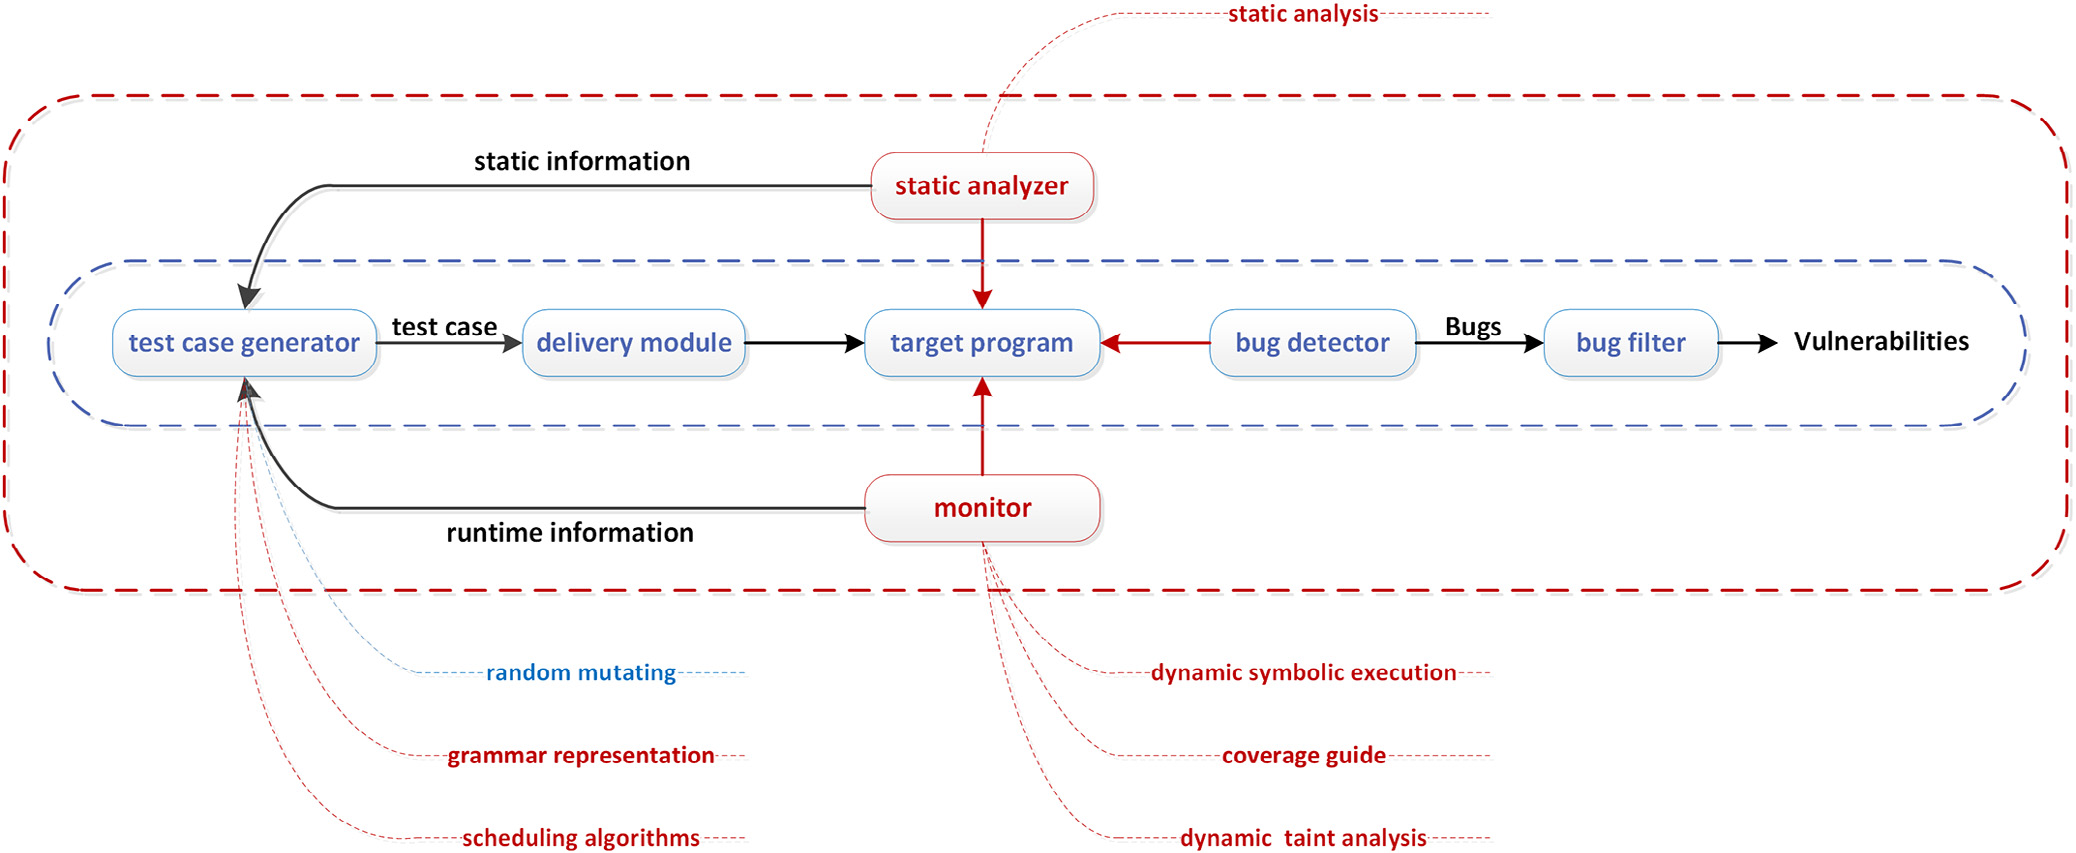
\includegraphics[width=0.9\textwidth]{assets/FuzzingSteps.jpg}
        \caption{Architectural Diagram of a Fuzzing System\cite{Science}}
        \label{fig:FuzzingSteps}
    \end{figure*}
    \subsubsection{Similarities Across Fuzzers}
    Since then, fuzzing systems have become more sophisticated and different techniques have been integrated. However, certain characteristics remain similar between all fuzzing systems. They output some concrete input(s) and configurations that can then be used to reproduce the fuzzer's observation, allowing confirmation, reproduction, and debugging of the discovered issues.\cite{EvaluatingFuzzTesting} They automatically find well-defined bugs, such as assertion errors, divisions by zero, \code{NULL} pointer dereferences, etc.\cite{AllYouEverWanted}

    \subsubsection{Architecture of a Fuzzer}
    \label{ArchitectureFuzzer}
    Figure\ref{fig:FuzzingSteps} shows the architecture of a typical fuzzer. Most fuzzers contain similar parts that are responsible for each step during the fuzzing process. These are explained below

    \paragraph{Target Program}
    The target program (also known as the program under test, or PUT) is the software to be tested. Different fuzzers have different requirements for the type of PUT they support: Some require access to the source code to add instrumentation during compilation, or because they work on an intermediate representation (IR), such as LLVM bytecode.

    \paragraph{Bug Detector}
    The bug detector watches the PUT during execution for illegal states. The simplest implementations trigger on program crashes, more sophisticated bug detectors might check if certain protected parts of the PUT are accessed, for example to check the implemented authentication.

    \paragraph{Bug Filter}
    The list of inputs that put a PUT into an illegal state may contain duplicates, in the sense that they exploit the same software defect. The bug filter attempts to deduplicate this list based on some heuristics such as stack hashes or the order in which basic blocks were executed.

    \paragraph{Test Case Generator}
    The task of the test case generator is to generate and select the next input to be tested. Based on the test case generator, fuzzing systems can be categorized as either mutation-based or generation-based. Mutation-based fuzzers take some inputs to the PUT as their input, and then repeatedly mutate them if the results produce \textquote{interesting} behavior\cite{EvaluatingFuzzTesting}.

    The prioritization is either random or based on a heuristic that assigns a value to each possible next input, which is used to select the next input to pass to the delivery module. Heuristics often take into account information produced by the monitor, such as coverage or distance to target instructions. These approaches can be further combined, for example, by alternating random and heuristic-based input selection.

    \paragraph{Delivery Module}
    The delivery module is responsible for passing the generated test case to the PUT in the expected form and triggering the actual execution. This can be as simple as running a command line utility with specified command line arguments, but can also include creating files to be accessed by the PUT, or even emulating user interaction.

    \paragraph{Monitor}
    Fuzzing systems can be further classified based on how much access the monitor module has to the PUT. Blackbox fuzzers make a single observation: whether or not the PUT has crashed. Graybox fuzzers have limited access to the PUT during execution. Typical information extracted by graybox fuzzers includes which basic blocks were executed in what order, or generally code coverage based on instruction, basic block, or statement. Whitebox fuzzers have full access to the PUT and allow sophisticated reasoning about program structure. Systems that use taint analysis or symbolic execution are categorized as whitebox fuzzers because they deeply examine the program structure during their analysis. Different systems make different tradeoffs, accepting higher analysis costs in the hope of better bug-finding effectiveness.\cite{EvaluatingFuzzTesting}

    \paragraph{Static Analyzer}
    The static analyzer, as its name suggests, attempts to extract information by statically examining the PUT's source code, IR or binary. Such information may include grammars accepted by the PUT or program paths that are considered high risk.

    \subsection{Symbolic Execution}
    \label{SymbolicExecution}
    The concept of symbolic execution in the context of program testing was introduced in \citeyear{Symbex} by \citeauthor{Symbex}.\cite{Symbex} By not executing a PUT with concrete values (such as the number \code{23} or the string \code{"Hello World!"}), but instead modelling certain or all values with mathematical variables, it allows to explore all possible paths of a program. Different engines (such as angr\cite{angr} or Triton\cite{Triton}) allow to perform symbolic execution on source code, an IR or a binary of a PUT.

    \subsubsection{Performing Symbolic Execution}
    During the execution of a given program, a symbolic execution engine computes and updates the so-called symbolic state with each instruction. It contains
    \begin{itemize}
        \item the inputs marked as symbolic as symbols $\alpha_i$,
        \item the symbolic expression store $\sigma$, which in turn contains
        \item symbolic expressions $\phi_j$, which are either a reference to a symbol $\alpha_i$ or an arithmetic combination of symbolic expressions, such as $\phi_j=\phi_k-\phi_l$, and finally
        \item the path constraint $\pi$, which is the conjunction of all branch constraints, i.e. the conditions on symbolic expressions to arrive at a certain point in the program, such as $\phi_1\leq2$ or $\phi_2=\phi_3\land\phi_4=3$.
    \end{itemize}

    During execution, the symbolic state changes according to the specific instruction being executed. If it performs some form of manipulation on existing data, this is represented by adding new symbolic expressions to the symbolic store. If a branch is (not) taken based on a check on variables or registers containing symbolic expressions, the path constraint is extended with an appropriate condition. The exploration of a program can follow different heuristics, such as breath- or depth-first search. Finally, the path constraint collected along certain paths can be formulated as a query to a Satisfiability Modulo Theory (SMT) solver. This solver can then prove whether the path associated with the constraint is reachable with \textit{any} input, and generate an input that directs the PUT execution in exactly the same way as the analyzed execution.

    \subsubsection{Categorizing Symbolic Execution Implementations}
    Symbolic execution implementations can be categorized in several ways: Where static dynamic execution exclusively and exhaustively executes the process described above, dynamic (or concolic, a portmanteau of \textquote{concrete} and \textquote{symbolic}) symbolic execution executes a program symbolically and with concrete values in parallel.

    Online symbolic execution allows multiple paths to be computed in parallel, while offline symbolic execution examines one path at a time. Finally, one can distinguish between partial and full symbolic execution, where only a part or all of the variables and therefore the computation is done symbolically.\cite{Ghidrion}

    \section{Methods}
    \label{Methods}

    Fuzzing is a extensively researched topic. For the search term \textquote{Fuzzing}, Web of Science\cite{WebOfScience} finds 2,741, Scopus\cite{Scopus} finds 2,410, and Google Scholar\cite{GoogleScholar} finds approximately 29,300 works. Even when filtered by the top places, summarizing the current state of symbolic execution in fuzzing from the ground up would be a task beyond the scope of this project.

    However, since fuzzing is such a well-published topic, other researchers have taken on the task of summarizing the state of the art, each group with a slightly different focus. These survey papers can therefore be used to approximate a complete picture of the current state of the art. This is the approach taken by the author of this paper. Section\ref{SurveyPapers} contains a list of the survey papers considered. To ensure accuracy and a consistent level of detail, the works discussed in these survey papers (primary works) are used to confirm or refute how the survey papers discuss the contributions of each primary work. However, the information in the review papers was generally trusted, and an in-depth analysis of each primary paper mentioned was beyond the scope of this work. Therefore, minor inaccuracies may have gone undetected.

    The following rules were applied when selecting review papers for inclusion in this work:
    \begin{itemize}
        \item First, various search engines were used to generate a list of survey papers in the field of fuzzing. Since even the amount of survey papers is overwhelming (Google Scholar\cite{GoogleScholar} returns more than 25,000 results for the search term \textquote{fuzzing survey}), works were only included if their title, abstract, or keywords contained the word section \textquote{fuzz} and if Google Scholar\cite{GoogleScholar} reports that they were cited more than 5 times or if they were published in a high-impact venue.
        \item Then, further review papers discussed, listed, or cited in other review papers were added (such as works listed in \cite{Demystifying}).
        \item Works published before January 1, 2010 (such as\cite{ViolatingAssumptionsWithFuzzing} or\cite{NewTrendsSymbex}) were not included to further limit the scope of this survey.
        \item Then, review papers focusing on a specific technique (such as machine learning\cite{ML1, ML2}) were excluded.
        \item Similarly, review papers focusing on hybrid fuzzing\cite{Hybrid, Exploratory} were discarded, since most hybrid fuzzers use symbolic execution only in a very limited fashion, which negates most of the obstacles faced by classical symbolic execution based fuzzers. However, to provide some introductory insight, a short survey paper on hybrid fuzzing\cite{SurveyHybrid} was selected to be included.
        \item In addition, works focusing on a specific use case for fuzzing, such as testing Internet of Things or other embedded devices\cite{IoT, Embedded, Embedded2}, network protocols\cite{Network, Network2023}, smart contracts\cite{Ethereum}, or JavaScript engines\cite{JavaScript, JavaScript2}, were excluded.
        \item Finally, a selection of additional works were added to the list based on the author's intuition.
    \end{itemize}

    \section{Related Work}
    \label{SurveyPapers}

    This section summarizes contributions of existing survey papers selected as described in Section\ref{Methods} and lists relevant primary works discussed in each. Primary works mentioned without discussion are omitted.

    \papertitle{AllYouEverWanted}
    Using a simple intermediate language (SIMPIL), this paper discusses taint analysis and forward symbolic execution, including examples and analysis of the theoretical foundations of symbolic execution. While fuzzing is mentioned in multiple instances, it is not the main focus. However, it still lists many of the drawbacks and advantages fuzzers based on symbolic execution have, and the additional perspective was valuable in assembling this review.

    \papertitle{PreliminaryAssessment}
    After giving a short overview of issues faced by symbolic execution based fuzzers, this paper focuses on eight high impact fuzzing tools (JPF-SE and Symbolic (Java) PathFinder\cite{JPFSE, JavaPathFinder}, DART\cite{DART}, CUTE\cite{CUTE} and jCUTE\cite{ExplicitPathModelChecking}, CREST\cite{CREST}, SAGE\cite{SAGE}, Pex\cite{Pex}, EXE\cite{EXE}, and KLEE\cite{KLEE}).

    \papertitle{FuzzingTheStateOfTheArt}
    \citeauthor{FuzzingTheStateOfTheArt} from Australia's Department of Defence provide an extensive look at fuzzing — \citetitle{FuzzingTheStateOfTheArt} is the longest of the discussed survey papers. After discussing the taxonomy, concepts, types, and history of fuzzing, they discuss a list of 15 works from scientific literature and ten commercial and open-source frameworks. In those scientific works, they present four papers that employ symbolic execution, namely KLEE\cite{KLEE}, SAGE\cite{SAGE}, GWF\cite{GWF}, and TaintScope\cite{TaintScope}.

    \papertitle{ReviewThreeDecades}
    This survey paper, as the title suggests, focuses on symbolic execution. Starting with an explanation of classical symbolic execution, it then provides a list of issues that fuzzing tools based on symbolic execution face, along with attempts to mitigate those by adapting and extending the algorithms. Finally, the authors present five high-impact tools they worked on: DART\cite{DART}, CUTE\cite{CUTE}, CREST\cite{CREST}, EXE\cite{EXE}, and KLEE\cite{KLEE}.

    \papertitle{Orchestrated}
    Orchestrated surveys \textquote{consist of a collaborative work collecting self-standing sections, each focusing on a key surveyed topic}\cite{Orchestrated}. One of the topics discussed in this particular work is symbolic execution. It contains short introductions into BBRBP\cite{BBRBP}, AGLT\cite{AGLT}, Darwin\cite{Darwin}, MATRIX RELOADED\cite{MATRIXRELOADED}, and SRA\cite{SRA} in its introduction. As mitigation strategies for path explosion, it discusses SMART\cite{SMART}, DDCSE\cite{DDCSE}, PFA\cite{PFA}, among others. For environment interaction, ASSIE\cite{ASSIE} and Cinger\cite{Cinger} are presented. Finally, to attempt to solve constraints that are too complex for direct SMT solver invocation, MCSS\cite{MCSS}, CORAL\cite{CORAL}, and its extension introducing AVM\cite{CORALAVM} are cited.

    \papertitle{Science}
    After discussing the structure of fuzzing systems and different targets observed in literature and industry, this paper focuses on inventions of primary works along the structure of fuzzers. Symbolic execution is discussed in the context of the sample generator and the monitor (see Section\ref{ArchitectureFuzzer}). Discussed primary works include CUTE\cite{CUTE}, KLEE\cite{KLEE}, SAGE\cite{SAGE}, TaintScope\cite{TaintScope}, BuzzFuzz\cite{BuzzFuzz}, GWF\cite{GWF}, Dowser\cite{Dowser}, BORG\cite{BORG}, Driller\cite{Driller}, and MoWF\cite{MoWF}. It further contains a sizeable section comparing symbolic execution based fuzzing systems and their contributions.

    \papertitle{FuzzingASurvey}
    \citeauthor{FuzzingASurvey} focus on coverage-guided fuzzing, mentioning other approaches that can be mixed in and different applications it can be used for. They further broadly discuss the challenges symbolic execution in fuzzing faces. Last, they present TaintScope\cite{TaintScope} and Driller\cite{Driller} as examples of using symbolic execution for specifically for path exploration.

    \papertitle{FuzzingStateOfTheArt2018}
    The first mention of a symbolic execution based fuzzer in this paper is SAGE\cite{SAGE}, which the authors use to summarize the limitations of whitebox fuzzing. In the following section, works bringing progress to a step in the fuzzing workflow are discussed, including SYMFUZZ\cite{SYMFUZZ}, TaintScope\cite{TaintScope} and KATCH\cite{KATCH}. Then, and most clearly relevant for this work, \citetitle{FuzzingStateOfTheArt2018} contains a discussion of the limitations of taint analysis and dynamic symbolic execution. Discussed works in this section include, among others,  SMART\cite{SMART}, HOTG\cite{HigherOrderTestGeneration}, Cloud9\cite{Cloud9}, APLS\cite{APLS}, SAGE\cite{SAGE}, CGF\cite{CGF}, DeepFuzz\cite{DeepFuzz}, TCR\cite{TCR}, DiSE\cite{DiSE}, and CRAXfuzz\cite{CRAXfuzz}.

    \papertitle{EvaluatingFuzzTesting}
    While not a classic survey paper, \citetitle{EvaluatingFuzzTesting} finds issues in how all 32 papers performed the evaluation of the system they introduced. It further proposes rules to follow to make an evaluation robust. Last, it contains a list of what advances each paper examined claims to introduce.

    \papertitle{HackArtScience}
    \citeauthor{HackArtScience} gives an easy-to-read introduction to fuzzing in this work. He distinguishes between blackbox, grammar-based, whitebox, greybox, and hybrid fuzzing and provides code examples that show how some of these approaches work. In the section about whitebox fuzzing, SAGE\cite{SAGE} is discussed comparatively extensively, KLEE\cite{KLEE}, S2E\cite{S2E}, and SPF\cite{SPF} are mentioned.

    \papertitle{SurveyHybrid}
    This fairly short paper focuses, as the title would suggest, on hybrid fuzzing — the combination of black-/greybox and whitebox fuzzing. Discussed work includes Hybrid Fuzz Testing\cite{HybridFuzzTesting}, Driller\cite{Driller}, QSYM\cite{QSYM}, SAVIOR\cite{SAVIOR}, and Pangolin\cite{Pangolin}.

    \papertitle{ChallengesAndReflections}
    Compared to other works, the authors of this article pursue a less technical and more conceptual approach to surveying the state of the art in fuzzing. They identify improvement areas such as usability, residual risk estimation, and fuzzer evaluation techniques and discuss current approaches and their limitations. To further legitimize their findings, they conducted a survey under security professionals from both academia and industry. The only symbolic execution based fuzzers mentioned are KLEE\cite{KLEE}, SAGE\cite{SAGE}, and Mayhem\cite{Mayhem}.

    \papertitle{ArtScienceEng}
    Starting with proposing a taxonomy for fuzzing itself and categorizing fuzzers, this paper proposes a general-purpose model of fuzzing, explaining the steps and approaches common fuzzers share. It further presents a genealogy, tracing the origins of important papers back to the work of \citeauthor{UNIX}. However, it \textquote{does not provide a comprehensive survey on DSE}\cite{ArtScienceEng}, but only discusses whitebox fuzzing in a subsection and refers to other survey papers such as \cite{Orchestrated, AllYouEverWanted} for a more complete overview.

    \papertitle{FuzzingASurveyforRoadmap}
    Similar to what is attempted in this paper, \citetitle{FuzzingASurveyforRoadmap} lists issues along common steps in fuzzing along with attempted solutions, but without the focus on symbolic execution. It does contain a short section about symbolic execution in the context input search space handling, but only discusses very few papers directly while often mentioning entire families of papers, with only some relying on symbolic execution.

    \papertitle{FuzzingVulnerabilityDiscoveryTechniques}
    After a short chapter on fuzzer classification, the main focus of this paper are steps and issues along a typical fuzzer workflow, told through the papers that made advances in each category. Finally, it presents current challenges in research and how they could be approached. The discussed papers include some that rely on symbolic execution: Angora\cite{Angora}, T-FUZZ\cite{TFuzz}, MoWF\cite{MoWF}, and HFL\cite{HFL}.

    \papertitle{SystematicReview2023}
    The authors of this paper guide the reader through advances in fuzzing along the works that introduced those. It includes a section about symbolic execution, which considers the following systems: Driller\cite{Driller}, QSYM\cite{QSYM}, SAVIOR\cite{SAVIOR}, DigFuzz\cite{DigFuzz}, Pangolin\cite{Pangolin}, and QuickFuzz\cite{QuickFuzz}.

    \papertitle{Demystifying}
    This paper dedicates one of its chapter to first explaining the fundamental logic of symbolic execution, and then presenting three implementations (Driller\cite{Driller}, CONFETTI\cite{CONFETTI}, and FUZZOLIC\cite{FUZZOLIC}). It further investigates advances in IoT firmware and kernel fuzzers, but does not explain where up- and downsides of using symbolic execution in these domains lay.

    \section{Challenges and Mitigation}
    \label{Results}
    This section focuses on attempts to mitigate inherent issues with symbolic execution. It categorizes the challenges and presents a (inexhaustive) list of works that introduced some improvement to deal with them. Many of the listed papers implemented further more general efficiency improvements, like SAGE's\cite{SAGE} (and multiple other papers inspired by it) generational search, which generates multiple new inputs from just one run of the symbolic execution engine by solving the constraint formula with the constraint from each branch flipped independently.

    \subsection{Environment Interactions}
    Within a symbolic execution environment, one can reason about program behavior, but this obviously breaks down when a program includes actions that interact with the real world and can not be modelled. Examples of this would be unhandled instructions, system calls, interrupts, inter-process communication like pipes or sockets, or interaction with external systems in general, since they might return unpredictable results because their logic is opaque to the symbolic execution engine.\cite{Demystifying} They might further introduce additional symbolic variables in their return values or have other side effects.

    \paragraph{Concolic Execution}
    Because of this, almost all systems examined perform some form of concolic execution. This allows them to simply use the concrete values whenever they encounter instructions that cannot be executed symbolically, acting as an exit whenever no other approach solves an issue. By using concrete values however, symbolic execution systems sacrifice completeness. But for any system that interacts with the environment in non-trivial ways, this usually is the only way to still test them. For non-emulatable function calls, parameters that are not influenceable by inputs — i. e. they are not symbolic — are just used directly, while values for symbolic variables are chosen randomly from the set of solutions to the current constraints on them.\cite{PreliminaryAssessment} Additionally, there are further advances that certain systems have made, which mean they do not have to drop down to concrete values but can evaluate more logic symbolically.

    \paragraph{Emulating Function Calls}
    One attempt to deal with system calls that is common across symbolic execution engines is to not perform system calls or even call to external libraries, but present the symbolic execution engine with code emulating their effects. This preserves the logical integrity of the resulting constraints and is often more efficient than the original library since it can rely on the operators understanding of the function's effect and does not rely on ways this logic has to be transformed to be executable by a machine. Examples for this technique would be EXE\cite{EXE} or KLEE\cite{KLEE}, and all other systems building on top of either of those (including PYGMALION\cite{PYGMALION}, KATCH\cite{KATCH}, and Cloud9\cite{Cloud9}).

    The downside of this approach is obvious: These summaries have to be created, maintained, and tested manually, while fuzzing systems generally strive to need as little operator interaction as possible. There are attempts to automatically infer input-output relational logic in the form of path constraint to be added for complex instructions based on executing it with many different values\cite{ASSIE}. Additionally, there are systems that analyze a PUT and prompt the operator to present models only for the program parts that actually introduce imprecision, like Cinger\cite{Cinger}.

    \paragraph{Kernel Fuzzing}
    HFL\cite{HFL} is a kernel fuzzer that heavily relies on symbolic execution. It lists three main issues the authors had to overcome: \textquote{(1) indirect control transfers determined by system call arguments (2) controlling and matching internal system state via system calls, and (3) nested argument type inference for invoking system calls}\cite{HFL}. To solve those issues, HFL \textquote{(1) converts implicit control transfers to explicit transfers, (2) infers system call sequence to build a consistent system state, and (3) identifies nested arguments types of system calls}\cite{HFL}.

    \subsection{Memory Modelling}
    As described in Section\ref{SymbolicExecution}, symbolic execution engines keep a memory representation of the process the PUT is running in in memory. However, modelling this memory poses a few challenges.

    \paragraph{Arithmetic}
    Operations on a physical machine differ from pure mathematical operations on symbolic expressions. For example, integers might over- or underflow. Modelling floating point arithmetic is even more difficult, since the imprecision introduced by rounding needs to be represented exactly in the resulting constraints to ensure accuracy. These issues are widely solved by symbolic execution engines by not representing numbers as mathematical numbers, but as bitmaps. The appropriate constraints then also need to be added on a bitmap level, thus introducing additional complexity. Certain engines further employ special constraint solvers that improve floating point based constraint handling (like FloPSy\cite{FloPSy}) and complex mathematical constraints (like CORAL\cite{CORAL} and its extension\cite{CORALAVM}).

    \paragraph{Symbolic Pointers}
    If an instruction performs a jump to a symbolic address, this presents a unique challenge to symbolic execution units, since this single operation increases the size the program's state space. This is a major scaling problem to the point of making calculations on any but the most trivial programs infeasible. The easiest, yet most inaccurate, way to deal with this challenge is to simply drop down to a concrete value, as described above, with the discussed downside of lost completeness. To maintain more than this base-level of accuracy, several strategies have been proposed.

    First, one can separate different operations on symbolic pointers. While dereferencing a symbolic pointer poses a challenge, comparing pointers might still be doable. Early adopters of this strategy included CUTE\cite{CUTE} and CREST\cite{CREST}, which only considers (in-)equality predicates with symbolic pointers. Both static analysis and solving the constraints on the symbol in question can potentially drastically reduce the amount of valid values it can take, thus reducing the amount of states needed to explore.

    EXE\cite{EXE} and KLEE\cite{KLEE} introduced the concept of regarding symbolic pointers as array accesses. An object accessed with a symbolic pointer is copied as often as necessary to model all possible results, including error states. Or, in other words, \textquote{a sound strategy is to consider it a load from any possible satisfying assignment for the expression}\cite{AllYouEverWanted}.

    While this works well if only one symbolic pointer is used, the situation becomes more complex once different symbolic pointers access the same data type from different parts of the program. This is because they might be accessing different or the same values, thus again creating a scaling problem by introducing many permutations. To deal with this issue (called memory aliasing), symbolic execution engines might perform alias analysis at run-time as in DART\cite{DART}. Other systems like Vin\cite{BitBlaze} optionally rewrite all memory addresses as scalars based on their name. While this is efficient, it is based on a potentially unsound assumption of variable name to value equality. Finally, certain SMT solvers (like STP\cite{STP} or Z3\cite{Z3}) can handle alias analysis, and can be used to delegate (some of) the work. This is done by, among others, EXE\cite{EXE}, KLEE\cite{KLEE}, and SAGE\cite{SAGE}.

    \subsection{Path Explosion}
    One of the primary issues symbolic execution faces is the so-called path explosion. This refers to the fact that the program path count is usually exponential in the number of static branches in the code. Because naïve symbolic execution attempts to emulate all possible branches, this requires an unobtainable amount of memory and compute resources for all but trivial programs. If examination is performed based on a simple depth-first search, it gets stuck in non-terminating loops with symbolic conditions and is therefore rarely used. Both EXE\cite{EXE} and KLEE\cite{KLEE} can however be configured to run in this mode.

    Symbolic execution, if implemented this way, can inherently help with path explosion, by only examining possible branches. An example: When running EXE\cite{EXE} on \code{tcpdump}, only 42\% of instructions contained symbolic operands, less than 20\% of of symbolic branches have both sides feasible.\cite{EXE}

    One simple approach is to set a user-defined timeout for the symbolic execution engine, after which approaches not based on symbolic execution are used. This is called hybrid fuzzing\cite{HybridFuzzTesting}. It is further discussed in Section\ref{HybridFuzzing}.

    Other than these, three main strategies are common: Reducing the search space, usage of advanced data structures and other optimizations to delay path explosion, and guiding the search to limit the effects of path explosion.

    \subsubsection{Search Space Reduction}

    Search space reduction can be performed in a few ways: First, \textquote{if a program path reaches the same program point with the same symbolic constraints as a previously explored path, then this path will continue to execute exactly the same from that point on and thus can be discarded.}\cite{RWset} This makes use of the fact that there are often multiple ways to get to the same program state by performing symbolic state analysis at runtime. Further optimizations on the basis of partial order and symmetry reductions were introduced by \citeauthor{GSE}.\cite{GSE}

    Similarly, MoWF\cite{MoWF} uses knowledge gained by its built-in blackbox fuzzer to prune invalid inputs and thus prevents its symbolic execution engine to get stuck in input checking and error handling code. CESE\cite{CESE} uses context-free grammars to limit its symbolic execution engine to interesting paths, as opposed to error handling during parsing. TCR\cite{TCR} intelligently reduces existing test cases and prioritizes the remaining according to heuristics to maximize exploration efficiency.

    \subsubsection{Using Advanced Data Structures}
    \label{AdvancedDataStructures}

    \paragraph{State Represantation} Since the symbolic state often only has minor differences between closely related paths, it can be represented by a data structure that allows copy-on-write. This means that only the changed parts actually need to be stored, reducing memory consumption significantly. Many systems employ this strategies: KLEE\cite{KLEE}, Mayhem\cite{Mayhem}, S2E\cite{S2E}, BORG\cite{BORG}, and Cloud9\cite{Cloud9}. States can also be merged statically, like in KLEE-FP\cite{KLEEFP}. To further lower pressure on memory, state information can be transferred to disk, like in Mayhem\cite{Mayhem}, BORG\cite{BORG}, and SAGE\cite{SAGE}. The latter also introduced a compact representation for path constraints.\cite{SAGE}

    \paragraph{Function and Data Structure Summaries} To limit the size of paths that need to exercised (and thus reducing the amount of symbolic expressions and the size of path constraints), functions can be analyzed and represented by a summary. These summaries can either be generated automatically, like in SMART\cite{SMART}, Higher Order Test Generation\cite{HigherOrderTestGeneration}, or Demand-Driven Compositional Symbolic Execution\cite{DDCSE}, or manually, as described by \citeauthor{PFA}\cite{PFA}. The latter also introduced a system where common complex structures like strings and regular expressions can be manually transformed into constraints.\cite{PFA} Using function summaries essentially reduces the problem of interprocedural paths to reasoning about intraprocedural paths. This was demonstrated in LATEST\cite{LATEST}.

    \subsubsection{Guiding the Execution}
    The approach to mitigating the path explosion problem receiving the most attention is execution guiding. It attempts to steer the execution to parts of the PUT that are interesting in an attempt to finish analysis (or at least produce findings) as soon as possible, thus reducing execution time before findings are produced to a bearable minimum.

    Since it is unknowable where exactly findings will be produced, search heuristics of varying complexity are employed to choose the next input to evaluate. These might take any number of inputs and trade off increased complexity for better precision.

    \paragraph{Dynamic Analysis} Most commonly, symbolic execution based fuzzers guide the execution by using the input which increases code (instruction, basic block, or statement) coverage. Examples include EXE\cite{EXE}, SAGE\cite{SAGE}, and CREST\cite{CREST}. Complementary, Fitnex\cite{Fitnex} is a state-dependent fitness function that measures distance between already discovered feasible paths is to a particular test target (as defined by any other heuristic).

    Other systems reward inputs that lead to longer runtime, (like in Automatic Generation of Load Tests\cite{AGLT}), or those that produce vastly different outputs based on very similar inputs, as in Symbolic Robustness Analysis\cite{SRA}. QuickFuzz\cite{QuickFuzz} weighs the approximate cost of executing a certain path against its demand and selects the next input based on this ratio.

    \paragraph{Static Analysis} The second group of attempts revolves around static analysis, usually in the form of examining the control flow graph (CFG) of a PUT. CREST\cite{CREST} \textquote{is an extensible platform for building and experimenting with heuristics for selecting which paths to explore}\cite{ReviewThreeDecades} and supports analysis of CFGs. This analysis might mark program parts as interesting based on different criteria and guide the execution towards these. GRT\cite{GRT} and VUzzer\cite{VUzzer} are examples of systems using general static analysis. Examples of more specific static analysis heuristics include the following:

    \begin{itemize}
        \item Directed Incremental Symbolic Execution\cite{DiSE}, Directed Test Suite Augmentation\cite{DTSA}, MATRIX RELOADED\cite{MATRIXRELOADED}, and KATCH\cite{KATCH} guide execution towards code that changed in a patch, thus using fuzzing as regression testing.
        \item Chopper\cite{Chopped} also uses code differences between two versions of a PUT to guide execution, but inverts the incentive structure: It ignores (resp. only lazily executes) certain functions deemed uninteresting to focus on certain parts of the PUT and prevent path explosion. While this designation could be done manually, Chopper\cite{Chopped} uses a heuristic which marks as uninteresting parts of the PUT which are far away from code changed in the examined patch.
        \item Darwin\cite{Darwin} uses symbolic execution to produce inputs that differ slightly from crashing inputs, which can then be used to triage and debug a certain software defect.
        \item CRAXfuzz\cite{CRAXfuzz} includes heuristics to determine interesting function calls like \code{malloc}.
        \item Dowser\cite{Dowser} looks for pointer dereferences in loops.
        \item SAVIOR\cite{SAVIOR} employs UndefinedBehaviorSanitizer\cite{UndefinedBehaviorSanitizer} to find potential bugs.
        \item BORG\cite{BORG} guides analysis towards buffer over-reads.
    \end{itemize}

    Alternatively, the approach can be inverted where execution is guided backwards from interesting parts of the PUT towards outer control structures, such as in DrillerGo\cite{DrillerGo}.

    \paragraph{Probabilistic Approaches}
    More recently, works have introduced approaches which employ heuristics to assign a probability to each potential next input and select which one to execute based on this value. DeepFuzz\cite{DeepFuzz} does this with the goal of finding inputs which will penetrate deeper into a PUT. MEUZZ\cite{MEUZZ} employs machine learning to examine potential next inputs and uses symbolic execution to validate the results. Finally, DigFuzz\cite{DigFuzz} uses Monte Carlo path optimization to quantify the difficulty of each path using grey-box fuzzing and then lets the white-box fuzzer focus on the paths that are believed to be most challenging for grey-box fuzzing to make progress.

    \subsection{Constraint Solving}
    \label{ConstraintSolving}
    For most fuzzing systems, constraint solving dominates the runtime. Thus, it is an area that received a lot of attention and several optimizations have been proposed, to make query evaluation faster and in some cases at all possible. They can be categorized as follows:

    \subsubsection{Query Optimization}
    \paragraph{Query Splitting} While solving the whole query might not be feasible, solving parts of it often is. This approach can be further separated in two approaches. The first attempts to identify independent sub-queries and solve them independently (implemented, among others, in EXE\cite{EXE} and KLEE\cite{KLEE}). This has the obvious limitation that even the smallest independent but internally interdependent parts of the query might still be too large to be solved. The second approach (implemented in Mixed Concrete-Symbolic Solving\cite{MCSS}) sacrifices some of its claim on completeness by solving parts of the query only and using the solution to solve the rest. This approach might produce false negatives, where there is a solution, but not with the results selected by the solver based on the first query.

    \paragraph{Query Reduction} Symbolic Execution often generates inefficient queries for the logic a certain function or program emulates. By using heuristics, such as pattern matching, multiple constraints can be reduced to a single constraint. However, while this approach shrinks the query passed to the SMT solver, it introduces a new scaling problem itself — the optimization passes for complex queries might consume an infeasible amount of time or resources, even to a point where solving the query without optimization is more efficient. Therefore, when introducing such heuristics systems need to carefully balance optimization and SMT solver execution time.

    The optimization might be executed either at the symbolic execution runtime afterwards on the complete query. Examples of the former are \textquote{loop-guard patterns matching rules to identify a constraint that defines the number of iterations of input-dependent loops during dynamic symbolic execution, then set new constraints representing the pre- and post-loop conditions to summarize sets of executions of that loop}\cite{Science}, as implemented in SAGE\cite{SAGE}, BORG\cite{BORG}, or APLS\cite{APLS}.

    Alternatively, using function summaries (as discussed in Section\ref{AdvancedDataStructures}) can also help to reduce the complexity of SMT queries, because the produced logic relationship between input and output is not bound to code and therefore the available instructions. On top of this, certain functions can be assigned only partial function summaries if they are only called with certain values, similar to mocks and stubs in unit testing. Moles\cite{Moles} provides a framework for this.

    Lastly, in certain context it might be beneficial to not use intermediate representation (IR) to execute on symbolically, but integrate the symbolic emulation with the native execution through dynamic binary translation, which prevents additional instructions (since often multiple RISC instructions in the IR are necessary to replace one CISC instruction), and allows finer-grained control over the constraint, thus making it smaller. This is done in QSYM\cite{QSYM}.

    \subsubsection{Using Information from Previous Queries}
    \paragraph{Exploiting Query Similarities} Since fuzzing systems based on concolic execution generate the next input based on the path the PUT executed under the previous input by flipping one of the constraints, there is a strong temporal relationship between consecutive constraint set and thus SMT queries. A solution to the first query is obviously known in the form of the input that initially produced the query. To solve the second, very similar, query, fuzzing systems can thus use parts of the first solution, since, if the part of the query they solve did not change, they might also solve the second query.

    This is a common approach, with subtle differences in implementations: SAGE\cite{SAGE} excludes parts of the query solved by previous results from the query passed to the SMT solver. CUTE\cite{CUTE} relies on a similar mechanism and adds an optimization that supersets of queries often do not invalidate existing solutions. An example of this would be when additional checks are performed in the PUT on a certain variable which was previously tested to be a valid input to the function under question further down the stack. Finally, KLEE\cite{KLEE} introduced a more versatile counterexample caching scheme for its SMT queries.

    \paragraph{Advanced Query Relationship Analysis}
    More recently, systems have introduced complex data structures to store their SMT queries, which then allow solvers to efficiently combine information gathered by previous invocations by exploiting the mathematical similarities between the queries. Pangolin\cite{Pangolin} for example uses polyhedral path abstraction to replace query parts for more efficient models based on prior results.

    \subsubsection{Improved SMT Solvers}
    While some of the improvements discussed above can be implemented in the fuzzers, a whole class of optimizations need to be implemented in the SMT solver. Because of this, improved SMT solvers were developed alongside many of the more influential symbolic execution based fuzzers. Because they are not part of the fuzzing systems themselves, they were not analyzed as part of this work. Nevertheless, the following SMT solvers are worth mentioning:

    Z3\cite{Z3} is one of the most powerful SMT solvers available today. It is developed at Microsoft and available open source under an MIT license and thus widely used, e.g. in SAGE\cite{SAGE} or angr\cite{angr} (which is used by Driller\cite{Driller}). Other SMT solvers used in symbolic execution based fuzzing include STP\cite{STP}, Yices\cite{Yices}, or cvc5\cite{CVC5} (which built during the development of EXE\cite{EXE}).

    \subsubsection{Alternatives to SMT Solvers}
    While the approaches listed above might improve the runtime of SMT solvers, they do not solve the fundamental problem in exponential complexity they face. A set of fuzzers therefore implement systems that allow them to reason about the relationship between input and program execution path without relying on SMT solvers. There is an argument to be made that these systems should no longer qualify as using symbolic execution since often their solutions are only approximate, but since their fundamental approach is similar and they are often listed next to symbolic execution based fuzzers in review papers, they are still discussed here.

    Fuzzers analyzing the dependency between input data and state space and approximating solutions to path constraints based on those to prevent expensive calls to an SMT solver are fairly common\cite{WEIZZ}:

    \begin{itemize}
        \item Intriguer\cite{Intriguer} uses taint analysis to discover instructions accessing a wide range of input bytes, and then performs symbolic execution for those instructions deemed important and only invokes the underlying SMT solver for complicated queries.
        \item Angora\cite{Angora} solves path constraints by using a combination of context-sensitive branch coverage, scalable byte-level taint tracking, gradient descent searching, input length exploration, and type and shape inference.
        \item Eclipser\cite{Eclipser} uses instrumentation on the PUT to generate partial path conditions, which can then be solved without invoking SMT solvers to generate further inputs.
        \item SMT formulas can be transformed into programs, which in turn can then be solved using a coverage-guided fuzzer to generate solutions to the initial formula. JFS\cite{JFS} uses this technique to find solutions to floating-point constraints.
        \item REDQUEEN\cite{REDQUEEN} exploits the fact that much of the input data ends up in the state-space and uses simple transformations on the input data as opposed to relying on taint analysis or symbolic execution to bypass checksums.
        \item Other proposals include approximate SMT solvers, such as FUZZY-SAT implemented in FUZZOLOGIC\cite{FUZZOLIC}, or optimistic SMT solvers, as in QSYM\cite{QSYM}.
    \end{itemize}

    \subsection{Handling Concurrency}
    Testing real-life concurrent programs in general is difficult because of their inherent non-determinism. This is also a challenge for symbolic execution based fuzzers. However, a few advancements have been made in this space: Generalized Symbolic Execution employs model checkers, who are able to handle multi-threading (and other forms of non-determinism). In general, \textquote{concolic testing was successfully combined with a variant of partial order reduction to test concurrent programs effectively.\cite{ScalableAutomatedMethods, OpenDistributedPrograms, ExplicitPathModelChecking, RaceDetection}}\cite{ReviewThreeDecades}

    One other development in the space of testing concurrent programs with symbolic execution was introduced in SPIN\cite{SPIN}: It allows checking if a concurrent program is equivalent to a sequential, less efficient, but less error-prone implementation of the same logic. It is used to check complex parallel numerical computations.

    \subsection{Recursive Data Structures}
    Similar to concurrency, recursive data structures are difficult to handle in any testing framework. In the space of symbolic execution fuzzers, GSE\cite{GSE} uses lazy initialization on recursive data structures. Pex\cite{Pex} supports inputs of primitive types as well as complex (i.e. recursive) data types. To handle the latter, Pex analyzes the PUT and generates factory methods for each. These invoke a constructor and a sequence of methods, with their parameters also determined by Pex' analysis.

    \subsection{Hybrid Fuzzing}
    \label{HybridFuzzing}
    Hybrid Fuzzing describes systems that combine multiple approaches to improving fuzzing's effectiveness. Many of these systems include components using symbolic execution. However, because they only selectively employ symbolic execution, many of the challenges described above are avoided altogether. As described in Section\ref{Methods}, hybrid fuzzing systems were only tangentially analyzed for this work. To still give readers an introduction, this section discusses a non-exhaustive list of hybrid fuzzing systems.

    \paragraph{Alternating Fuzzing Types} Tools like Driller\cite{Driller} perform black- or greybox fuzzing (in the case of Driller using AFL\cite{AFLPlusPlus}) until they are \textit{stuck}, meaning they are unable to produce inputs that discover additional paths. Driller then, and only then, invokes its concolic execution engine (Driller uses angr\cite{angr}) to trace the program under investigation executed with one of the previously generated inputs and generate a new input based on the collected path constraint that reaches a section of the PUT Driller was previously unable to reach. Because Driller does not use symbolic execution for its primary discovery tool, it does not suffer from issues such as path explosion, because it only ever executes one path at a time using symbolic execution.

    Other systems interleaving black-/greybox and symbolic execution based fuzzing are Hybrid Concolic Testing\cite{HCT} and Cyberdyne\cite{Cyberdyne}. DrillerGo\cite{DrillerGo} uses a similar approach, but specifically targets \textquote{unsafe system calls or suspicious locations, or functions in the call stack of a reported vulnerability that we wish to reproduce}\cite{DrillerGo}. Other targeted hybrid fuzzing systems include 1dVul\cite{1dVul} or BugMiner\cite{BugMiner}.

    \paragraph{PUT Manipulation} By removing code blocks that are deemed irrelevant, T-FUZZ\cite{TFuzz} prevents its mutation-based fuzzer (which does not use symbolic execution) from getting stuck. It then employs symbolic execution to validate the bugs found. TaintScope\cite{TaintScope} uses taint analysis to bypass checksum checks and then symbolic execution to fix checksum fields in malformed test cases. Similary, Stinger\cite{Stinger} analyses a PUT and then only employs symbolic execution on the parts of the PUT that contribute to path constraints. Like this, the overhead introduced by a symbolic execution engine can be limited to parts of the program.

    \paragraph{High-Quality Test Input Generation} IFL\cite{IFL} generates quality input to a smart contract based on a symbolic execution engine and then uses them to train a neural network. This can then be used to fuzz other smart contracts since they often implement similar functionality.

    PYGMALION\cite{PYGMALION} uses symbolic execution to generate a grammar from a program, generates valid inputs from that, and finally uses those in fuzzers (AFL\cite{AFLPlusPlus} and KLEE\cite{KLEE}) to measure the achieved code coverage. AUTOGRAM\cite{AUTOGRAM} accomplishes a similar goal of producing a context-free grammar a PUT accepts by executing it with different inputs based on taint analysis.

    \paragraph{Other Uses of Symbolic Execution} SYMFUZZ\cite{SYMFUZZ} uses symbolic execution to determine the optimal mutation ratio from a given program-seed pair. If a program by a software vendor crashes an a customer's device, BBRBP\cite{BBRBP} generates new inputs that do not or at least to a lesser extent contain private information. To achieve this, the instructions executed if a program is fed the initial crashing input are recorded, and then run using symbolic execution. Finally, the generated path constraint is solved by an SMT solver, which produces a new, unrelated input.

    \section{Future Work}
    \label{FutureWork}
    This work marks only the beginning of what information can be extracted from the combination of review papers and primary works discussed in this work or even in this field in general. What follows is a list of ideas for further analyses.

    \subsection{Additional Review Papers to Consider}
    Section\ref{Methods} mentions different criteria, according to which survey papers were excluded from this work. However, they might still contain important information missed by excluding them. Specifically, certain works appeared to early\cite{AutomaticTestDataGeneration, BruteForceVulnDiscovery,BreakingSoftware}, or focus on symbolic execution based software testing, but do not primarily concern fuzzing\cite{DSETestGeneration, SurveySymbex, SearchStrategies, NewTrendsSymbex, ReviewConcolicTesting}.

    \subsection{Bibliometry}
    Survey papers might collectively be a good way to measure the importance of primary papers. By carefully selecting survey papers, looking at their bibliography, and counting how often each primary paper appears, one could get a measurement of importance for each. To ensure fairness, the scores would need to be weighted based on how many review papers were written after their publication date.

    Compared to examining the bibliographies of primary papers, works which introduced a new technique copied or adapted by many subsequent works would likely be less heavily weighted. This would skew the results to works highly influential based on their outcomes and ongoing development, not only the techniques they introduced.

    By doing time-based analysis, one might even be able to distinguish between works that are still relevant today, as opposed to works which were made redundant soon after their publication by other works implementing the same approach more successfully.

    Finally, analyzing the context, in which a certain citation appears might further improve accuracy of a bibliometric score of the importance of a primary work. If it is only mentioned, it could be deemed less important compared to if it is discussed extensively. Instead of complex linguistic analysis, counting how often a source is cited or examining the section they appear in might serve as an imperfect but easier to implement substitution.

    \subsection{Author Analysis}
    While reading the survey papers discussed in Section\ref{SurveyPapers}, one thing that became apparent is that some review papers were (co-)written by authors of important primary works. One example is Cristian Cadar, who is the author of EXE\cite{EXE}, KLEE\cite{KLEE}, KLEE-FP\cite{KLEEFP} RWset\cite{RWset}, KATCH\cite{KATCH}, EGT\cite{EGT}, Chopped\cite{Chopped}, and JFS\cite{JFS} and co-wrote review papers\cite{ReviewThreeDecades, ChallengesAndReflections, PreliminaryAssessment}.

    This is to be expected, since these authors already know the matter at hand very well. But it might also mean that their own work is over-represented in the review papers they helped assemble. By investigating this relationship, one might gain insight into how easy or hard it is to gain recognition as authors new to this field. It may also serve as a measure of how likely it is that innovative works by new authors are missed by review papers.

    \subsection{Genealogy}
    Since most works discussed in this paper introduce improvements in a specific part of a fuzzing system, they often rely on an existing system for the rest and extend it. One example is PYGMALION\cite{PYGMALION}, KATCH\cite{KATCH}, and Cloud9\cite{Cloud9} building on top of KLEE\cite{KLEE}, APLS\cite{APLS} extending SAGE\cite{SAGE}, or CRAXfuzz\cite{CRAXfuzz} extending S2E\cite{S2E}, which in turn again extends KLEE\cite{KLEE}.

    Building a genealogy tree from the primary works discussed might provide a list of highly adaptable and stable projects, which might in turn be better suitable for deployment in commercial applications. \citetitle{ArtScienceEng}\cite{ArtScienceEng} contains a diagram of such a genealogy. However, since this work does not focus on symbolic execution based fuzzing, it does not distinguish between nuances withing this subfield and only includes a limited amount of projects, while \citetitle{Hybrid}\cite{Hybrid} focuses on hybrid fuzzing systems only.

    Further, if not extending the code itself, ideas or concepts introduced by a paper might get copied or adapted by subsequent work. Building a genealogy dataset across these might uncover hidden relationships between projects and show the importance of ideas implemented in fuzzers across the board.

    \subsection{Meta-Survey}
    Finally, one could compare review papers based on different categories: primary works discussed (see above), categorizations of fuzzers, or more specifically categorization of problems that symbolic execution in fuzzing faces and the solutions to them that different works propose.

    \section{Conclusion}
    \label{Conclusion}
    This survey presents an introduction into fuzzing, specifically the use of symbolic execution in fuzzing systems, its challenges and innovations. It includes discussion of the theoretical foundation of both fuzzing in general and symbolic execution specifically, and explains how these two approaches to software testing were combined to create state-of-the-art systems.

    Because this field has received extensive attention from both academia and industry, survey papers on fuzzing are used to collect significant works, including summaries and discussion of them. First, the focus of each of the 17 selected survey paper is summarized, along with a list of 78 discussed symbolic execution based fuzzers. The latter are then combined, extended, and categorized. The resulting list shows that a diverse set of attempts has been made to mitigate each inherent challenge of symbolic execution, thus making it usable on real-world programs.

    Finally, this work reflects on its own approach of using existing survey papers to gather information about a certain fields. Both limitations during this process and possible additions to this work are discussed. By using this approach, an infeasibly big research area was penetrated, yielding an extensive overview of the state of the art in symbolic execution based fuzzing.

    \defbibheading{bibliography}[\bibname]{\section*{#1}}
    \addcontentsline{toc}{section}{\bibname}
    \printbibliography

    % \renewcommand{\thesubsection}{\arabic{subsection}}
    % \renewcommand{\thesubsubsection}{\arabic{subsection}.\arabic{subsubsection}}
    % \setcounter{subsection}{0}
    % \setcounter{subsubsection}{0}
    % \section*{Appendix}
    % \addcontentsline{toc}{section}{Appendix}
\end{multicols}

\end{document}
